\section{Plan}
\label{sec:sec004}

We will evaluate {\it BreastScreening-AI} simulating real-world conditions with 10 clinicians of \hyperlink{https://hff.min-saude.pt/}{Hospital Fernando Fonseca}.
Our goal will be to quantitatively and qualitatively assess the proposed design principles that the {\it BreastScreening-AI} system embodies (rather than on particular widgets of the UI) and to understand how these principles would fare in practice.
We will be particularly interested in understanding how {\it BreastScreening-AI} would accomplish improvements of diagnosis, surpassing the challenges and providing evidence of the opportunities emerging from HAII.
Ultimately, we will focus on clinicians' accuracy while using our {\it BreastScreening-AI} features and how to improve AI reliability during medical decision-making.

\subsection{Framework}
\label{sec:sec00401}

The proposed {\it BreastScreening} framework (Figure~\ref{fig:fig008}) will incorporate an {\it AI-Assisted} tool offering clinicians a second opinion during the breast cancer diagnosis that will be accomplished using a DenseNet model~\cite{chen2019learning}.
To validate the proposed DenseNet results, our framework allows the radiologist to {\it accept} or {\it reject} the proposed BI-RADS classification.
Therefore, the clinician can freely control the final diagnosis result.
The {\it BreastScreening} platform operates as a website that can be accessed via a web browser.

\footnotetext[2]{\hyperlink{https://cornerstonejs.org/}{cornerstonejs.org} - a {\it JavaScript} library to display interactive medical images including but not limited to DICOM. It was used to display the medical images on the browser.}

%%%%%%%%%%%%%%%%%%%%%%%%%%%%%%%%%%%%%%%%%%%%%%%%%%%
\begin{figure}[h]
\centering
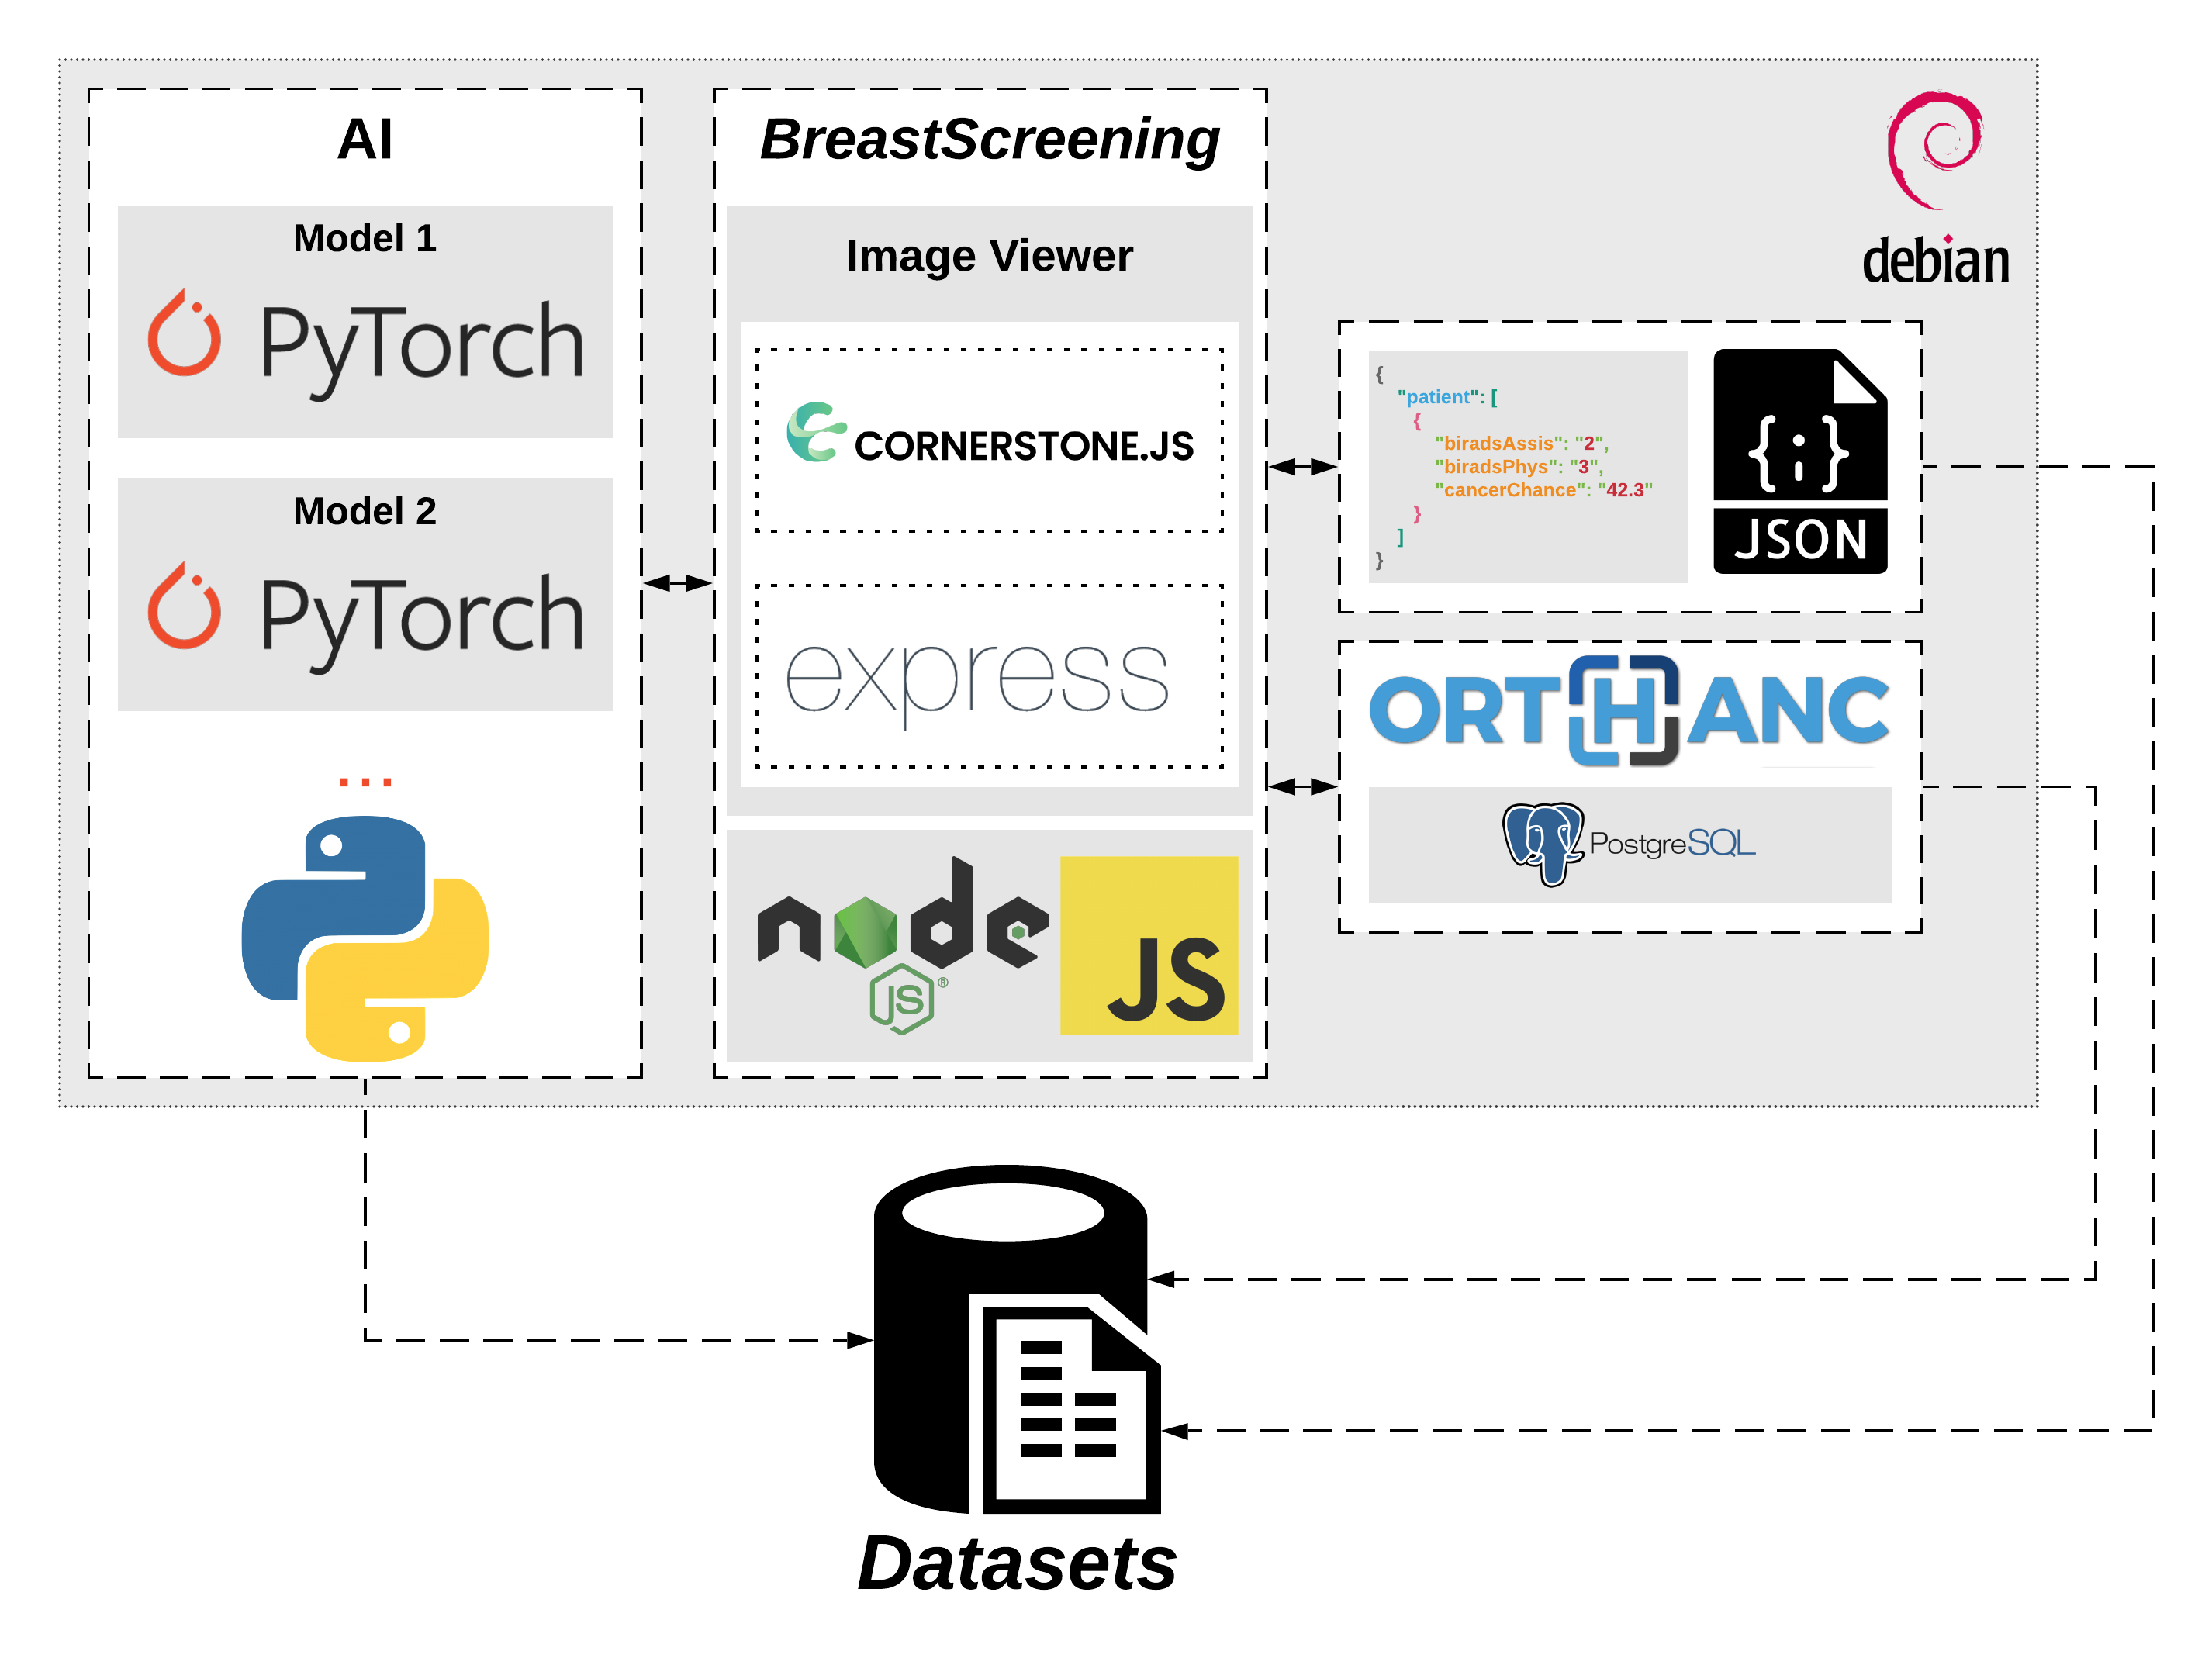
\includegraphics[width=0.45\textwidth]{fig008}
\caption{{\it BreastScreening-AI} Architecture: the main components of the system are AI Application, Image Viewer, Datasets and DICOM Storage. The Image Viewer of {\it BreastScreening} framework will provide essential interaction tools for clinicians. A study list is fetched from the Orthanc server, and through CornerstoneJS the radiologist can manipulate the image, interacting with the assistant at the same time.}
\label{fig:fig008}
\end{figure}
%%%%%%%%%%%%%%%%%%%%%%%%%%%%%%%%%%%%%%%%%%%%%%%%%%%

\subsection{Implementation}
\label{sec:sec00402}

{\it BreastScreening} framework will be implemented using {\it CornerstoneJS}\footnotemark[2]~\cite{urban2017lesiontracker} with a {\it NodeJS} framework\footnotemark[3]~\cite{10.5555/3002437, drnasin2017javascript} and {\it ExpressJS}\footnotemark[4]~\cite{10.1117/12.2285952} for managing the server part.
To feed the system, we will select image sets from \hyperlink{https://hff.min-saude.pt/}{Hospital Fernando Fonseca} and upload them into an {\it Orthanc} server~\cite{Jodogne2018}.
Three imaging modalities (MG, US and MRI) will be provided for each patient.
The images will be pre-processed and anonymized on the {\it Orthanc} server and then consumed by the system.
This system, needs to be efficiently designed as a set of modules (Figure~\ref{fig:fig008}) that can be reused in other imaging applications.

\footnotetext[3]{\hyperlink{https://nodejs.org}{nodejs.org} - a {\it JavaScript (JS)} based framework for back-end implementation. {\it NodeJS} is defined as a {\it JS} code execution environment.}

\footnotetext[4]{\hyperlink{https://expressjs.com}{expressjs.com} - minimal and flexible {\it NodeJS} web application framework that provides a robust set of features. It deals with requests, responses and subsequent middleware functions.}

\subsection{Study Setup}
\label{sec:sec00403}

For the study, we will conduct both quantitative and qualitative analysis.
The quantitative analysis will focus on measuring the clinicians' performance ({\it e.g.}, number of False-Positives and False-Negatives) during diagnosis of three groups of patients ({\it i.e.}, low, medium and high severity) for each doctor.
The above measurements are part of the quantitative analysis with a comparison between Assertive and Non-Assertive scenarios.
With that comparison, we will answer the  research questions and hypothesis mentioned in Section~\ref{sec:sec00305}, providing evidence for the impact, expectations and acceptance of {\it AI-Assistance} on the radiology room workflow.
For the qualitative analysis, we will extract opinion-based feedback from recorded audios.

\subsection{Procedure}
\label{sec:sec00404}

At this stage, each participant will interact with the assistant, {\it accepting} or {\it rejecting} the system suggestion in the two different scenarios.
The set of patients will provide participants with 289 patients, while all patients must have at least one of the three available modalities.
Each participant will open the respective set of three patients ({\it e.g.}, {\bf P1}, {\bf P2} or {\bf P3}), chosen randomly, and will examine the set of images.
During the examination, the participant will interact with the available features of the system.

\subsection{Measures}
\label{sec:sec00405}

We will measure system accuracy through three questions adapted from the Model of Trust~\cite{schoorman2016perspective} that we called Dimensions Of Trust Scale (DOTS).
The three questions will be answered on a 20-point scale with 5\% increments.
Furthermore, we will do several {\it post-task} questions.
The {\it post-task} questions, aim to evaluate satisfaction.
We will also measure the recall and precision ({\it e.g.}, through the FP and FN rates) of the system.

\break